\documentclass[letterpaper, oneside]{book}
%\usepackage{lingmacros}
\usepackage{tree-dvips}
\usepackage{amsmath}
%\usepackage{listings}
%\usepackage{graphicx}
%\usepackage{xcolor}
\usepackage{mdframed}
\usepackage{fancyhdr}
\usepackage[export]{adjustbox}
\usepackage[skip=10pt]{parskip}
\usepackage{amsfonts}
\usepackage{hyperref}
\usepackage{algorithm}
\usepackage{algpseudocode}
\usepackage{amsthm}
\usepackage{amssymb}
\pagestyle{plain}

\theoremstyle{definition}
\newtheorem{definition}{Definition}[chapter]
\theoremstyle{remark}
\newtheorem*{remark}{Remark}

\newtheorem{theorem}{Theorem}[chapter]
\newtheorem{corollary}{Corollary}[theorem]
\newtheorem{lemma}[theorem]{Lemma}
\newtheorem{prop}{Proposition}[chapter]

\graphicspath{{./images/}}

\begin{document}

\chapter{Quadratic Programming}

\section{Quadratic Optimization Problem}

In this chapter, we will present a brief introduction to Quadratic Programming.

Quadratic programming is a set of methods that solves a class of optimization problem with quadratic form. More specifically, we want to minimize the following objective function
\begin{displaymath}
	c^{\mathsf{T}}x + \frac{1}{2}x^{\mathsf{T}} \Sigma x
\end{displaymath}

subject to the following constraints:
\begin{displaymath}
	a_i^{\mathsf{T}}x \leqslant b_i, \quad i=1,2,...,m
\end{displaymath}

In the above expression, $x \in \mathbb{R}^n$ is the variable, $c \in \mathbb{R}^n$ is a constant vector, and $\Sigma \in \mathbb{R}^{n\times n}$ is a constant matrix. The optimization problem has $m$ constraints and for all $i$, $a_i \in \mathbb{R}^n$ and $b_i \in \mathbb{R}$.

The constraints can be expressed in a more compact form:
\begin{displaymath}
	Ax \leqslant b
\end{displaymath}
where 
\begin{align*}
	A^{\mathsf{T}} & = [a_1 \, a_2 \, ... \, a_m] \;\; \textrm{and} \\
	b^{\mathsf{T}} & = [b_1 \, b_2 \, ... \, b_m]
\end{align*}

Note that  $A$ is a matrix in $\mathbb{R}^{m \times n}$ and $b$ is a vector in $\mathbb{R}^n$. Vector $a_i$ is called a constraint vector.

An constraint $i$ is active if $a_i^{\mathsf{T}}x = b_i$. A related concept -- active constraints indices -- is defined as follows:
\[
	I(x_0) = \{i \ | \ a_i^{\mathsf{T}}x_0=b_i\}
\]

Note that the size of $I(x_0)$ is bounded by the number of constraints. In other words,
\[
	|I(x_0)| \leqslant m
\]

The set of points that satisfy all the constraints forms feasible region of the optimization problem, denoted by $\mathcal{R}$.

One of the key concepts in quadratic programming is quasi-stationary point, which is defined as follows:

\begin{definition}[Quasi-Stationary Point]\label{def_quasi_stationary_point}
	The point $x_0$ is quasi-stationary if $x_0\in \mathcal{R}$, and $x_0$ is optimal for the problem
	\begin{displaymath}
		\textrm{min}\{c^{\mathsf{T}}x + \frac{1}{2}x^{\mathsf{T}}\Sigma{}x \;|\; a_i^{\mathsf{T}}x=b_i, \;\forall i \in I(x_0)  \}
	\end{displaymath}
\end{definition}

The point $x_0$ is a nondegenerate quasi-stationary point if it's a quasi-stationary point and the gradients of those constraints active at $x_0$ are linearly independent. The point $x_0$ is a degenerate quasi-stationary point if it's a quasi-stationary point and the gradients of those constraints active at $x_0$ are linear dependent.

\begin{remark}
	An extreme point (in the context of linear programming) is a special case of quasi-stationary point. Recall that the $x_0$ is an extreme point if $x_0 \in \mathcal{R}$ and there are $n$ constraints having linearly independent gradients active at $x_0$. This reduces $I(x_0)$ to a single point, which is also the optimal point.
\end{remark}
\begin{prop}
	There are at most $2^m$ quasi-stationary points.
\end{prop}

\begin{proof}
	There are $m$ constraints so the number of all subsets of the $m$ constraints is $2^m$. It follows that there are $2^m$ sub optimization problems in the definition \ref{def_quasi_stationary_point} and each of them produces either zero or one quasi-stationary point.
\end{proof}



\section{Building Blocks}

We can now present the main constructs in Quadratic Programming. The algorithm moves from one quasi-stationary point to another and always decreases the objective function. As there are a finite number of quasi-stationary, the process will eventually terminate.

Moving from one quasi-station point to another requires finding the correct direction. This process is guided by the lemma below:

\begin{lemma}\label{lemma_search_direction}
	Let $x_0$ satisfy $Ax_0 = b$. Then $x_0 - s_0$ is optimal for $min\{ c^{\mathsf{T}}x + \frac{1}{2} x^{\mathsf{T}}\Sigma{}x \;|\; Ax = b \}$ if and only if $s_0$ satisfies the linear equation:
	\begin{displaymath}
		\begin{bmatrix}
			\Sigma{} & A^{\mathsf{T}} \\
			A & 0
		\end{bmatrix}		
		\begin{bmatrix}
			s_0\\
			v_0
		\end{bmatrix}
		= 
		\begin{bmatrix}
			g_0 \\
			0
		\end{bmatrix}
	\end{displaymath}
	where $g_0 = \nabla{}f(x_0)$. The first matrix is generally denoted by
	\begin{displaymath}
		H = \begin{bmatrix}
			\Sigma{} & A^{\mathsf{T}} \\
			A & 0
		\end{bmatrix}
	\end{displaymath}
\end{lemma}

\begin{remark}
	The condition here is different from the optimality conditions. In the optimality conditions, the coefficients are required to be positive, i.e. $v_i \ge 0$. In the lemma above, there is no such requirement.
\end{remark}

\begin{remark}
	it's intentional that the coefficient vector is cal $v_0$ instead of $u_0$. The difference is that for an optimization problem with equality constraints, the optimality condition only requires $\nabla f(x_0)  = A^{\mathsf{T}} v$ and the sign of the components does not matter. On the contrast, the optimality condition of an optimization problem with inequality constraints takes the following forms:
	\begin{align*}
		-\nabla f(x_0) = A^{\mathsf{T}} u \quad \mathrm{and} \quad \forall i, u_i \geqslant 0
	\end{align*}
\end{remark}

\begin{lemma}\label{lemma_full_row_rank}
	Suppose matrix $A$ has full row rank. Then $H$ defined in the previous lemma is non singular.
\end{lemma}

\section{Quadratic Programming Algorithm}
The quadratic programming adopts an iterative approach. The algorithm starts with a feasible point $x_0 \in \mathcal{R}$.

Let $A_0$ denote the submatrix of $A$ corresponding to those constraints active at point $x_0$.

\begin{center}
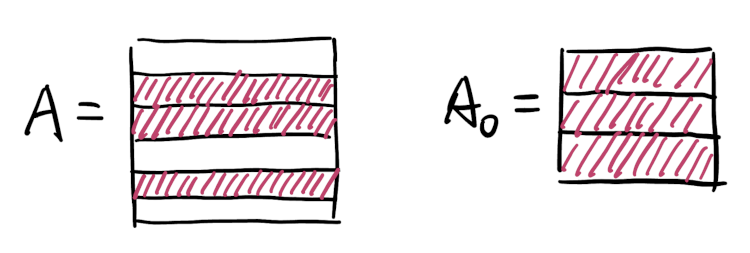
\includegraphics[width=0.6\textwidth]{matrix_a_and_a0_small.png}
\end{center}

Let $b_0$ denote the corresponding subvector of vector $b$. By definition, we have

\begin{displaymath}
	A_0 x_0 = b_0
\end{displaymath}

In this document, we assume matrix $A_0$ has full row rank so that we can use lemma \ref{lemma_full_row_rank}. 

Let 
\begin{displaymath}
	H_0 = 
	\begin{bmatrix}
		\Sigma{} & A_0^{\mathsf{T}} \\
		A_0 & 0
	\end{bmatrix}	
\end{displaymath}

Since $H_0$ is invertible under the assumption, we can solve the linear equation in \ref{lemma_search_direction} and determine the value of $s_0$. Recall that $s_0$ is the search direction, the next step is to determine the step size. Let $\sigma$ be a non-genative scalar and consider the following function:

\begin{displaymath}
	\sigma: \; \mapsto f(x_0 - \sigma s_0)
\end{displaymath}

It can be shown that the above function is a decreasing function for $0 \leqslant \sigma \leqslant 1$ and attains its minimum at $\sigma = 1$. The problem is that $x_0 - s_0$ may not be feasible anymore.


\begin{center}
	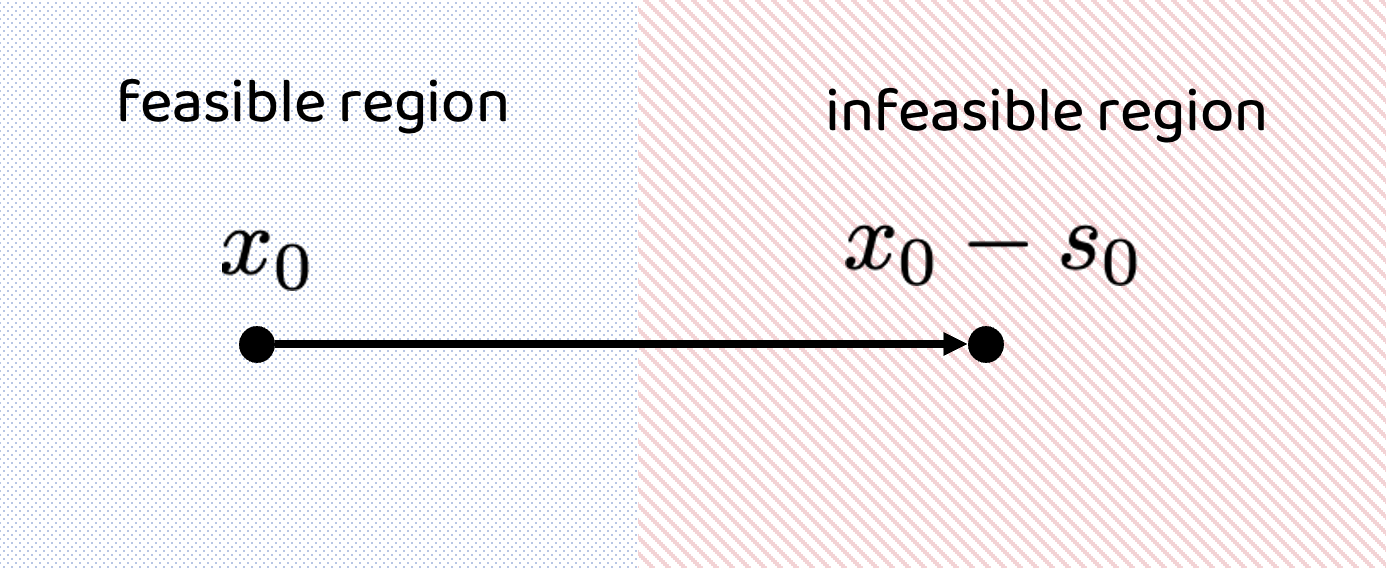
\includegraphics[width=0.6\textwidth]{search_direction.png}
\end{center}

Let's determine the conditions for the point $x_0 - \sigma s_0$ to satisfy all constraints. In other words, for any constraint $i$, we have

\begin{align*}
	a_i^{\mathsf{T}}(x_0 - \sigma s_0) \leqslant b_i \\
	\Rightarrow -\sigma a_i^{\mathsf{T}} s_0 \leqslant b_i - a_i^{\mathsf{T}}x_0
\end{align*}

If $a_i^{\mathsf{T}}s_0 \ge 0$, then constraint $i$ is satisfied automatically because the left side is negative and the right side is positive ($x_0$ is in the feasible region so it satisfies the constraint). 

If $a_i^{\mathsf{T}}s_0 < 0$, then 
\begin{displaymath}
	\sigma \leqslant \frac{b_i - a_i^{\mathsf{T}}x_0}{-a_i^{\mathsf{T}}s_0}
\end{displaymath}

It follows that the maximum step size is
\begin{displaymath}
	\hat{\sigma} = \min \left\{ 
	\frac{b_i - a_i^{\mathsf{T}}x_0}{-a_i^{\mathsf{T}}s_0}, \;\; \mathrm{for}\; i \; \mathrm{such}\;\mathrm{that}\; a_i^{\mathsf{T}}s_0 < 0
	\right\} 
\end{displaymath}

Since there is a finite number of constraints, let $l$ denote the index that attains minimum and $\sigma_0$ be the maximum distance. In other words,

\begin{displaymath}
	\hat{\sigma} = \frac{b_l - a_l^{\mathsf{T}}x_0}{-a_l^{\mathsf{T}}s_0}
\end{displaymath}

\begin{center}
	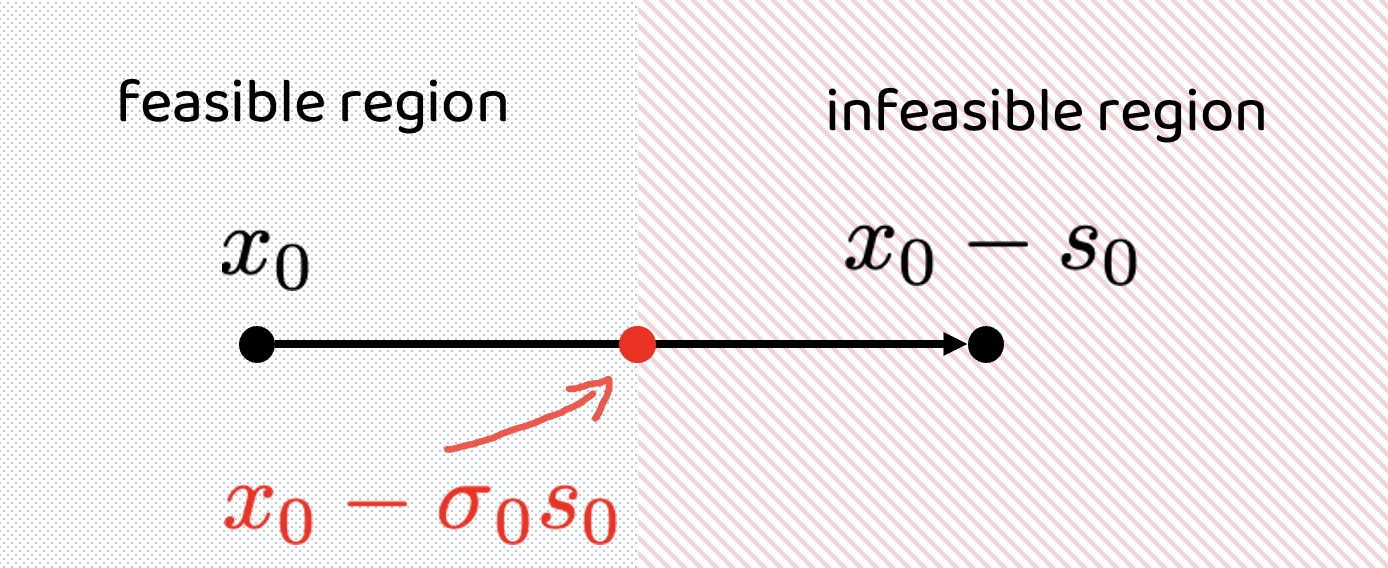
\includegraphics[width=0.6\textwidth]{maximum_step_size.png}
\end{center}

There are two cases to handle. To simplify our discussion and notation, define $x_1 = x_0 - \sigma_0 s_0$.

\textbf{Case 1}: $\sigma_0 < 1$

In this case, some previously inactive constraints has become active at $x_1$ and the index of this constraint is $l$. We can now add this constraint to the matrix $A_0$ and repeat the process. 

Note that $a_l$ cannot be linearly dependent on the columns of $A_0^{\mathsf{T}}$. This can be shown by contradiction. Suppose $a_l$ is linearly dependent on the columns of $A_0^{\mathsf{T}}$. There exists a vector $\omega$ such that

\begin{align*}
	& A_0^{\mathsf{T}} \omega  = a_l \\
	\Rightarrow \quad & s_0^{\mathsf{T}}(A_0^{\mathsf{T}} \omega) = s_0^{\mathsf{T}} a_l \\
	\Rightarrow \quad & (A_0 s_0)^{\mathsf{T}} \omega  = s_0^{\mathsf{T}} a_l
\end{align*}

By construction(\ref{lemma_search_direction}), $A_0 s_0 = 0$. It follows that
\[ 
	s_0^{\mathsf{T}} a_l = 0
\] 

which contradicts the definition of index $l$ because by definition, $a_l^{\mathsf{T}}s_0 < 0$.

This process cannot continue forever because the dimension of the matrix $A_0$ is finite. At some point, we need to deal with the second case.

\textbf{Case 2}: $\sigma_0 = 1$.

In this case, $x_1 = x_0 - s_0$ and the gradient is given as
\begin{align*}
	& g_1 = c + \Sigma x_1 \\
	& \quad = c + \Sigma (x_0 - s_0) \\
	& \quad = c + \Sigma x_0 - \Sigma s_0 \\
	& \quad = g_0 - \Sigma s_0 \\	
	\Rightarrow \quad & g_0  =  g_1 + \Sigma s_0
\end{align*}

According to lemma \ref{lemma_search_direction}, 
\[
H_0	
\begin{bmatrix}
	s_0\\
	v_0
\end{bmatrix}
= 
\begin{bmatrix}
	g_0 \\
	0
\end{bmatrix}
\]

Expanding the first row, we obtain

\begin{align*}
	& \Sigma s_0 + A_0^{\mathsf{T}} v_0 = g_0 \\
	\Rightarrow \quad & g_1 = A_0^{\mathsf{T}} v_0
\end{align*}

Now construct a new matrix $A_1$ by deleting the constraint where the coefficient is negative. Suppose this constraint has index $k$. For simplicity, let's further assume the following relationship holds:
\[
	A_0^{\mathsf{T}} = [A_1^{\mathsf{T}} \; a_k]
\]

Now we have
\[
	g_1 = [A_1^{\mathsf{T}} \; a_k] v_0
\]

Multiplying the equation by $s_1$, we obtain
\[
	g_1^{\mathsf{T}} s_1 = v_0^{\mathsf{T}} 
	\begin{bmatrix}
		A_1 s_1\\
		a_k^{\mathsf{T}} s_1
	\end{bmatrix} = 
	\begin{bmatrix}
	0\\
	a_k^{\mathsf{T}} s_1
	\end{bmatrix}
	= -u_k(a_k^{\mathsf{T}} s_1)
\]

Therefore, we have 
\[
	-g_1^{\mathsf{T}} s_1 = u_k(a_k^{\mathsf{T}} s_1)
\]

It can be shown by Taylor's theorem that $g_1^{\mathsf{T}} s_1 > 0$ and by definition $u_k < 0$, therefore 
\[
	a_k^{\mathsf{T}}s_1 > 0
\]

Now we can show the constraint $k$ is not active for the point $x_1 - \sigma  s_1$:
\begin{align*}
& a_k^{\mathsf{T}} (x_1 - \sigma s_1) = a_k^{\mathsf{T}} x_ 1 - \sigma a_k^{\mathsf{T}}s_1 \\
\Rightarrow \quad & a_k^{\mathsf{T}} x_ 1 - a_k^{\mathsf{T}} (x_1 - \sigma s_1) = \sigma a_k^{\mathsf{T}}s_1 
\end{align*}

Because $k$ was an active constraint, we have $a_k^{\mathsf{T}} x_ 1 = b_k$. Both $\sigma$ and $a_k^{\mathsf{T}}s_1$ are positive number, we conclude
\[
b_k - a_k^{\mathsf{T}} (x_1 - \sigma s_1) > 0
\]

\section{Summary}
\begin{center}
	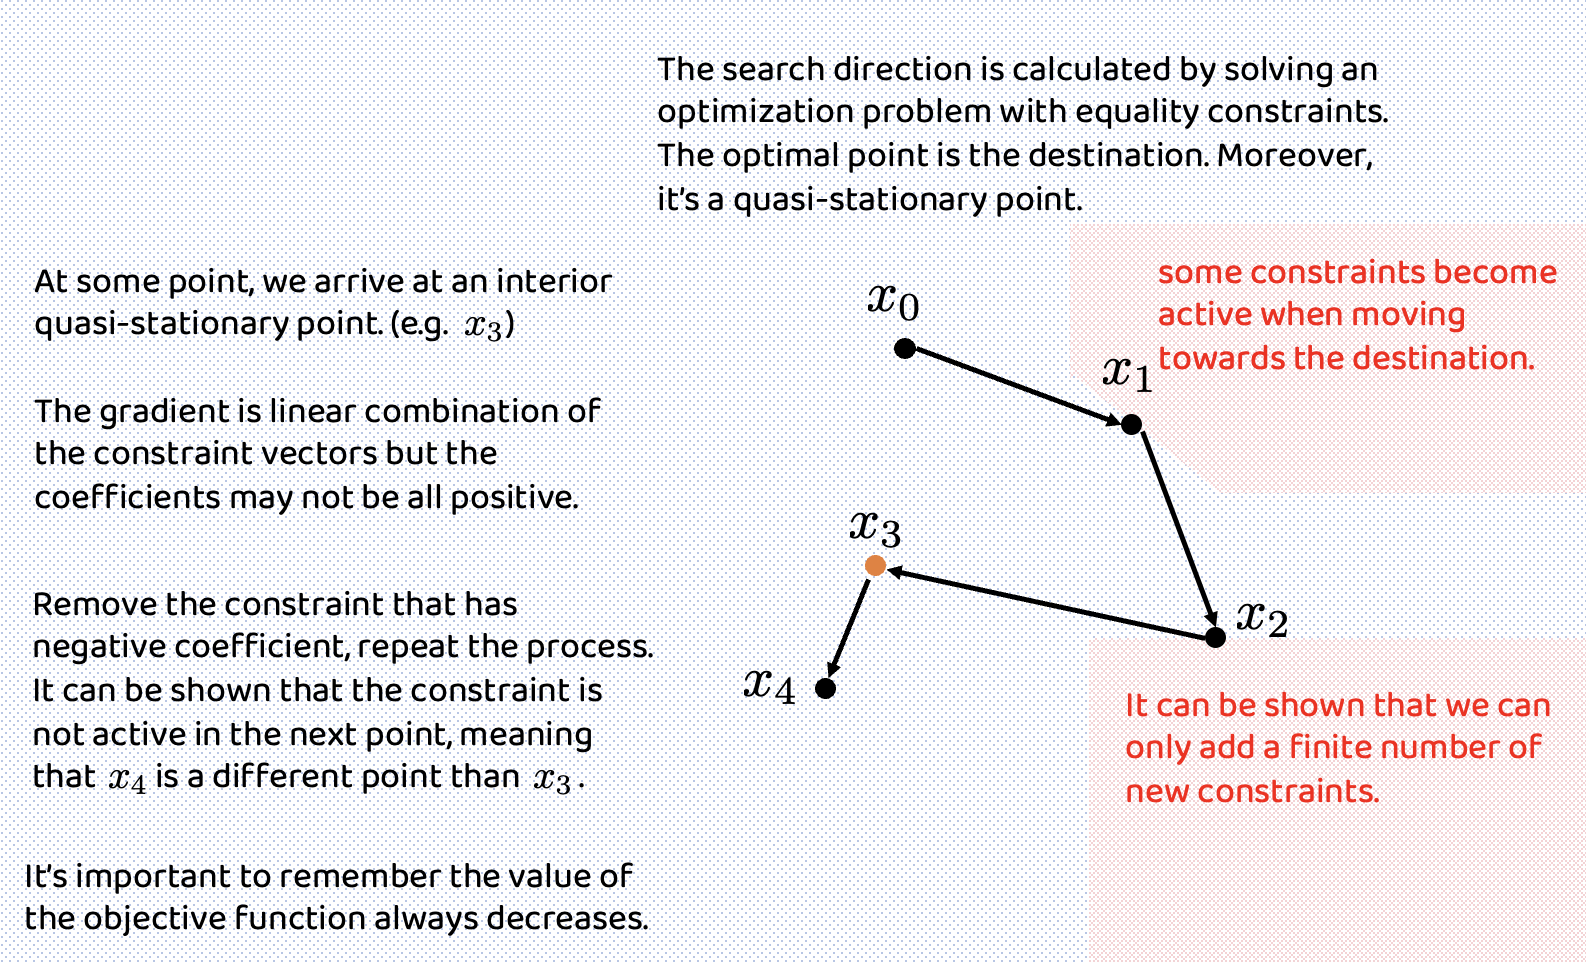
\includegraphics[width=0.9\textwidth]{summary_of_process.png}
\end{center}


\end{document}